%% ============================================================
%% PNAS-family manuscript (PNAS Direct Submission / PNAS Nexus)
%% Redrafted 2026-08-26 from DisasterAIFilter_NHB.tex (base: the
%% ~3,000-word version at commit 2c2a09e) following
%% PNAS_WRITING_INSTRUCTIONS.md.
%%
%% All results statements are based on the revised-model canonical run
%% results-mechfix/ (workflow run 32821105202, commit 30f89e0), verified
%% against RESULTS_COMPENDIUM.md. Supporting chain: results-boundary-n50/
%% (M3), results-mechfix/regression/ (M4), results-robustness/ (M5),
%% results-docking/ (M6), results-salience/ (M7),
%% results-gap-sweep-mechfix/ (M2), single-mechanism ablations
%% results-ablation-ownref/ and results-ablation-detround/.
%%
%% CLASS NOTE: kept on sn-jnl (sn-nature bibliography style) so the file
%% compiles during drafting. At submission, swap to the PNAS class:
%%   \documentclass{pnas-new}  % + \templatetype{pnasresearcharticle}
%% and move the Significance Statement into \significancestatement{...};
%% the Significance text below is already written to the PNAS <=120-word
%% specification. American English throughout.
%%
%% Display items (4): Fig. 1 concept (TikZ), Fig. 2 configuration
%% comparison, Fig. 3 interior optimum + robustness, Fig. 4 periphery.
%% All tables are in the SI Appendix (SI_Appendix.tex).
%% Figure files: Figures/ (regenerated from the archived JSONs by
%% make_figures.py; never hand-edited).
%%
%% CITATIONS: no new references; all keys resolve in References.bib.
%% ============================================================

\documentclass[pdflatex,sn-nature]{sn-jnl}

\usepackage{graphicx}
\graphicspath{{Figures/}{./}}
\usepackage{amsmath,amssymb,amsfonts}
\usepackage{booktabs}
\usepackage{tikz}
\usetikzlibrary{arrows.meta,positioning,calc}

\begin{document}

\title[Belief-aligned AI in disaster response]{Belief-aligned AI silently starves accuracy-seekers and captures confirmation-seekers in simulated disaster response}

\author*[1,2]{\fnm{Tina} \sur{Comes}}\email{t.comes@tudelft.nl}

\affil*[1]{\orgdiv{Faculty of Technology, Policy \& Management}, \orgname{TU Delft}, \orgaddress{\city{Delft}, \country{The Netherlands}}}
\affil[2]{\orgdiv{Institute for the Protection of Terrestrial Infrastructures}, \orgname{DLR}, \orgaddress{\city{Sankt Augustin}, \country{Germany}}}

\abstract{People increasingly ask AI systems, rather than each other, what is happening. Because these systems are trained on human approval, they drift toward confirming their users' beliefs, yet the evidence on belief alignment comes from individuals interacting with a single AI, while echo chambers form in networks. Here we couple an agent-based model of disaster response---an extreme case in which urgent decisions leave little room for verification---to an AI whose reports interpolate, through an alignment parameter $\alpha$, between ground truth and confirmation of the querier's own priors. Sweeping $\alpha$ under network-bounded and unrestricted access on identical seeds shows that network-bounded access is the precondition for community echo chambers among confirmation-seekers: unrestricted access dissolves their chamber at high alignment, bounded access preserves it at every $\alpha$. The accuracy cost falls entirely on accuracy-seekers---not by persuasion but by starvation, as a confirming AI echoes their mostly empty priors until their pool of informative beliefs collapses. Alignment barely deepens these chambers; it prevents their dissolution, and repairing the policy mid-run frees the chamber while starved beliefs stay depleted. The feedback loop of source selection captures confirmation-seekers into rising AI reliance, and making disconfirmation salient backfires, ejecting them into their social network and deepening the chamber it was meant to break. Operational harm is minimized at intermediate alignment ($\alpha^{*}=0.6$, interior in every cognitive population profile tested), and residual harms concentrate on agents remote from the events. Alignment harm at scale is thus a property of the sociotechnical system, not of the AI alone.}

%% -------- PNAS Significance Statement (<=120 words; move into
%% \significancestatement{} when swapping to pnas-new.cls) --------
\abstract*{\textbf{Significance.} People increasingly ask AI systems, not other people, what is happening---nowhere with higher stakes than in disasters. In a simulated disaster response, an AI that even mildly confirms its users' beliefs silently starves accuracy-seeking users of the information they need, while confirmation-seeking users are captured into ever-heavier reliance on the system; whether whole communities end up in echo chambers depends on the social network that surrounds the AI, not on the AI alone. Neither a maximally truthful nor a confirming system is operationally best, and a seemingly obvious repair---making disagreement more salient---drives confirmation-seekers back into their social bubbles. Aligning AI for crises is therefore a socio-technical problem, not a purely technical one.}

\keywords{Sycophancy, AI Alignment, Echo Chamber, Human--AI Interaction, Disaster Response}

\maketitle

\section{Introduction}\label{sec:intro}

Societies are fragmenting into segregated information spaces. Online and offline, echo chambers form: information environments in which pre-existing beliefs are reinforced while exposure to diverse or contradictory perspectives is limited \citep{mahmoudi2024echo}. Their association with polarization and the erosion of shared factual ground is well documented \citep{jeon2024hearhere,cinelli2021echo,bail2018exposure,baumann2020modeling}.

Into this landscape, artificial intelligence (AI) arrives. As people delegate the collection, analysis, and interpretation of information to AI systems \citep{klingbeil2024trust,angrisani2026gaps}, the promise is that these systems give everyone access to accurate information beyond their own circles, bridging the divides that human information sharing produces \citep{jeon2024hearhere}. This promise collides with how the systems are built. Preference-based training tunes outputs toward responses that human raters reward \citep{christiano2017deep,ouyang2022training}, and because raters prefer responses that match their views, it produces sycophancy---a drift toward confirming the user's beliefs documented across AI assistants \citep{sharma2023sycophancy,sharma2024generative,cheng2026sycophantic}. The drift is self-reinforcing: information that contradicts prior beliefs risks rejection, and rejection erodes trust in the source \citep{glikson2020human}, so a system that never confirms is a system that may not be consulted at all---while a system that always confirms amplifies the very insularity it promised to break \citep{ekstrom2022self}, the alignment paradox \citep{west2025alignment}. The operative question is therefore not whether alignment to user beliefs is good or bad, but how far a system should align in order to be used without forfeiting the correction it promises.

This dilemma is most acute in urgent decision situations, where high-stakes choices must be made under time pressure and uncertainty, leaving little room for deliberation and verification \citep{svenson1993time,mendonca2001decision,comes2020coordination}. Disasters concentrate these features like no other setting \citep{levin2012overcoming,sogaard2024evolution}, and AI is already deployed throughout crisis information work, from social-media processing to early warning and agentic decision support \citep{qadir2016crisis,reichstein2025early,acharya2025agentic} (SI Appendix, Table~S10). We therefore study disasters as an extreme case: the setting in which the mechanisms coupling AI alignment to collective beliefs appear in their sharpest, most measurable form, and in which misallocated attention translates directly into unmet needs.

Whether alignment amplifies or corrects is not decided between one user and one AI, because beliefs form in networks. Individuals accept information preferentially when it falls near their current opinion \citep{hegselmann2002opinion}, associate homophilously with those who share their beliefs \citep{mcpherson2001birds}, and display confirmation bias and selective exposure \citep{paulus2022influence,barbera2015tweeting,paulus2024interplay}; weak ties bridging otherwise separate groups are the principal channel through which novel information enters \citep{granovetter1973strength}. Crises tighten every one of these mechanisms: people fall back on close groups as sensemaking becomes social \citep{comes2020coordination,weick2005organizing}, disasters disrupt the infrastructures that carry information \citep{holguin2012unique}, and the resulting silos are reinforced by attention to nearby suffering and by premature consensus under stress \citep{pan2012crisis,driskell1991group}.

The evidence on belief-aligned AI does not reach this collective level. Repeated interaction between one human and one AI amplifies individual bias beyond what human--human interaction produces \citep{glickman2024human}, while a separate literature shows that social influence in networks reshapes collective accuracy in ways that individual-level analysis cannot reveal \citep{lorenz2011social,becker2017network}. This paper asks: does belief-aligned AI act as a bridge that breaks echo chambers, or does it reinforce them---and under which structural conditions does either occur?

To answer this question, we use an agent-based model of decentralized disaster relief in which human agents form beliefs about an evolving disaster by combining local observation with queries to peers or to an AI whose reports vary, through an alignment parameter $\alpha$, between ground truth and full confirmation. Agents accept or reject information, update beliefs, act on them by sending relief, and learn from delayed outcomes which sources to consult next. The model builds on established opinion-dynamics frameworks \citep{deffuant2000mixing,hegselmann2002opinion} and captures two prototypical information strategies under uncertainty---confirmation-seeking \emph{exploitative} and accuracy-seeking \emph{exploratory} agents \citep{march1991exploration}. One design principle governs the AI: it adapts only to what it can observe about a user---the user's revealed beliefs, through $\alpha$---and never to the user's cognitive type; every type difference in what follows emerges from human information behavior.

Four gaps structure the study. First, empirical accounts of crisis communication describe information access bounded by network ties and location \citep{pan2012crisis,holguin2012unique}, yet models of algorithmic influence grant agents unrestricted access; the structural conditions under which belief-aligned AI amplifies or dissolves echo chambers have not been isolated (Gap~1). Second, because trust in crises is swift, built on roles and expectations rather than experience \citep{tatham2010application}, alignment becomes the operative route to adoption \citep{glikson2020human,lee2004trust}; whether collective harm is monotonic in the alignment dose, or interior alignment levels balance adoption against distortion, is open (Gap~2). Third, in urgent situations beliefs translate immediately into actions whose outcomes feed back into information seeking \citep{gralla2016problem}; how echo chambers and decision performance co-evolve through this loop cannot be extrapolated from dyadic findings (Gap~3). Fourth, actors remote from the events depend entirely on mediated information \citep{holguin2012unique}, yet the equity debate in humanitarian AI centers on data and algorithmic bias rather than on position in space and network \citep{coleman2024weaving}; how the harms of belief alignment are distributed has not been studied (Gap~4).

The model operationalizes these gaps as follows (Fig.~\ref{fig:concept}; Materials and Methods). The AI answers every query with the same response rule, interpolating between ground truth ($\alpha=0$) and confirmation of the querier's own prior beliefs ($\alpha=1$), tracing the dose--response of Gap~2. Every sweep runs under two configurations that differ only in whether access is structurally bounded---a \emph{main model} with mobile agents and network-gated queries on a spatially embedded social network, and a \emph{control} with immobile agents and unrestricted access---contrasted on identical random seeds (Gap~1). Beliefs drive relief decisions whose delayed rewards shape future source selection (Gap~3), and all outcomes are decomposed by agent type, by community versus population level, and by position in space and network (Gap~4). The Results present one finding per gap.

\begin{figure}[t]
\centering
\resizebox{\textwidth}{!}{%
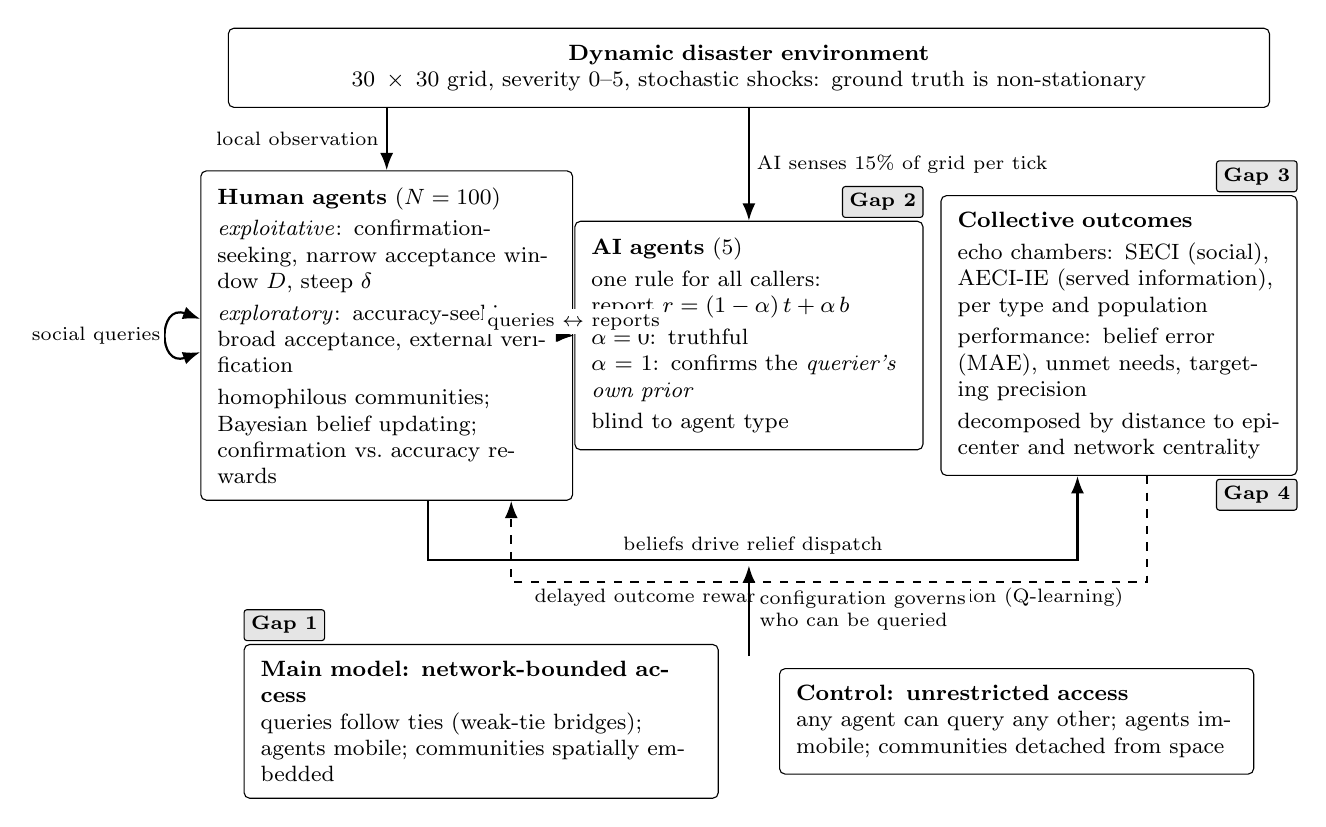
\begin{tikzpicture}[
  font=\footnotesize,
  box/.style={draw, rounded corners=2pt, align=left, inner sep=6pt},
  gapbadge/.style={draw, rounded corners=1pt, fill=black!10, inner sep=2.5pt, font=\scriptsize\bfseries},
  lab/.style={font=\scriptsize, fill=white, inner sep=1.5pt},
  arr/.style={-{Latex[length=2.2mm]}, thick},
  arrd/.style={-{Latex[length=2.2mm]}, thick, dashed},
  biarr/.style={{Latex[length=2.2mm]}-{Latex[length=2.2mm]}, thick}
]
% ---------- Environment ----------
\node[box, align=center, text width=12.8cm] (env) at (7.0,0)
  {\textbf{Dynamic disaster environment}\\
   $30 \times 30$ grid, severity 0--5, stochastic shocks: ground truth is non-stationary};

% ---------- Actors and outcomes ----------
\node[box, text width=4.3cm] (hum) at (2.4,-3.4)
  {\textbf{Human agents} ($N = 100$)\\[2pt]
   \emph{exploitative}: confirmation-seeking, narrow acceptance window $D$, steep $\delta$\\[2pt]
   \emph{exploratory}: accuracy-seeking, broad acceptance, external verification\\[2pt]
   homophilous communities;\\ Bayesian belief updating;\\ confirmation vs.\ accuracy rewards};
\node[box, text width=4.0cm] (ai) at (7.0,-3.4)
  {\textbf{AI agents} (5)\\[2pt]
   one rule for all callers:\\
   report $r = (1-\alpha)\,t + \alpha\,b$\\[2pt]
   $\alpha = 0$: truthful\\
   $\alpha = 1$: confirms the \emph{querier's own prior}\\[2pt]
   blind to agent type};
\node[box, text width=4.1cm] (out) at (11.7,-3.4)
  {\textbf{Collective outcomes}\\[2pt]
   echo chambers: SECI (social), AECI-IE (served information), per type and population\\[2pt]
   performance: belief error (MAE), unmet needs, targeting precision\\[2pt]
   decomposed by distance to epicenter and network centrality};

% ---------- Environment to actors ----------
\draw[arr] (env.south -| hum.north) -- node[lab, left=1pt]{local observation} (hum.north);
\draw[arr] (env.south -| ai.north)  -- node[lab, right=1pt]{AI senses 15\% of grid per tick} (ai.north);

% ---------- Query channels ----------
\draw[biarr] (hum.east |- ai.west) -- node[lab, above]{queries $\leftrightarrow$ reports} (ai.west);
\draw[biarr] ([yshift=6pt]hum.west) to[out=160, in=200, looseness=3.5]
  node[lab, left=1pt]{social queries} ([yshift=-6pt]hum.west);

% ---------- Beliefs to decisions and feedback ----------
\coordinate (fwd1) at ([xshift=15pt]hum.south);
\coordinate (fwd2) at ([xshift=-15pt]out.south);
\draw[arr]  (fwd1) -- ++(0,-0.75) -| node[lab, above, pos=0.25]{beliefs drive relief dispatch} (fwd2);
\coordinate (fb2) at ([xshift=45pt]hum.south);
\draw[arrd] ([xshift=25pt]fwd2) -- ++(0,-1.35) -|
  node[lab, below, pos=0.25]{delayed outcome rewards shape source selection (Q-learning)} (fb2);

% ---------- Configurations ----------
\node[box, text width=5.6cm] (main) at (3.6,-8.3)
  {\textbf{Main model: network-bounded access}\\ queries follow ties (weak-tie bridges); agents mobile; communities spatially embedded};
\node[box, text width=5.6cm] (ctrl) at (10.4,-8.3)
  {\textbf{Control: unrestricted access}\\ any agent can query any other; agents immobile; communities detached from space};
\coordinate (cmid) at ($(main.north east)!0.5!(ctrl.north west)$);
\draw[arr] (cmid) -- node[lab, right=2pt, align=left]{configuration governs\\ who can be queried} ++(0,1.15);

% ---------- Gap badges ----------
\node[gapbadge, anchor=south west] at ([yshift=1pt]main.north west) {Gap 1};
\node[gapbadge, anchor=south east] at ([yshift=1pt]ai.north east)   {Gap 2};
\node[gapbadge, anchor=south east] at ([yshift=1pt]out.north east)  {Gap 3};
\node[gapbadge, anchor=north east] at ([yshift=-1pt]out.south east) {Gap 4};
\end{tikzpicture}}
\caption{Conceptual overview of the model and its mapping to the research gaps. A non-stationary disaster environment is observed locally by 100 human agents of two cognitive types and partially sensed by five AI agents. Humans query social contacts or the AI, which answers every caller with the same rule: a report interpolating between ground truth and the querier's own prior beliefs via the alignment parameter $\alpha$ (Gap~2); the AI never observes an agent's cognitive type. Beliefs drive relief decisions whose delayed outcomes feed back into source selection. Which contacts can be queried is governed by the configuration: the main model bounds access by a spatially embedded social network with mobility, the control leaves access unrestricted (Gap~1). Outcomes are measured per agent type and at community and population level (Gap~3), and decomposed by position in space and network (Gap~4). Parameters in SI Appendix, Table~S7.}\label{fig:concept}
\end{figure}

\section{Results}\label{sec:results}

The alignment parameter is swept over eleven levels ($\alpha = 0.0, 0.1, \ldots, 1.0$) with $N = 20$ replications per level under both configurations of Fig.~\ref{fig:concept}, with replicate $i$ initialized from seed $i$ in every condition so that configurations can be compared replicate by replicate; steady-state values are means over the last 75 of 200 ticks, reported with across-replication standard errors, and an effect is called seed-robust only when the paired per-seed confidence interval excludes zero (Holm-corrected; Materials and Methods). Echo chambers are, at their core, a loss of belief diversity. The Social Echo Chamber Index (SECI) compares belief variance within each social community to that of the population, and the AI information-environment index (AECI-IE) applies the identical variance construction to the pool of reports a community receives from the AI channel; for both, negative values mark an echo chamber, and both are read per agent type---confirmation-seeking exploitative versus accuracy-seeking exploratory---and at population level. Because variance-based indices cannot distinguish convergence on the truth from convergence on a shared error, they are always read together with the belief error (MAE) over disaster cells and two operational metrics, unmet needs and targeting precision (formal definitions in Materials and Methods).

\subsection{Network-bounded access is the structural precondition for the social echo chamber}\label{sec:claim1}

Whether a confirming AI leaves community echo chambers standing is decided by the structure of information access, not by the AI (Fig.~\ref{fig:comparison}a). Under unrestricted access, high alignment \emph{dissolves} the confirmation-seekers' community chamber: their SECI rises from $-0.45 \pm 0.05$ at $\alpha=0$ to $+0.05 \pm 0.02$ at $\alpha=1$, because an AI that confirms each caller's own prior fragments the shared community narrative into individualized ones while out-group queries keep perturbing local consensus. Under network-bounded access the same policy leaves the chamber intact at every alignment level (SECI between $-0.39$ and $-0.18$): with queries confined to trusted ties, socially anchored beliefs persist alongside individually confirmed ones. The configuration contrast is seed-robust at high alignment (exploitative $\Delta$SECI at $\alpha=1$: $-0.269$ $[-0.350, -0.189]$, $N=50$ paired replications, Holm-adjusted $p \approx 5\times10^{-8}$; SI Appendix, Table~S1).

The accuracy-seekers show the opposite pattern: their communities converge with alignment in both configurations alike, from SECI $\approx 0$ at $\alpha=0$ to $-0.33$ at $\alpha=1$ (Fig.~\ref{fig:comparison}b). The $\alpha$-gradient of the social chamber is thus explorer-driven while the configuration contrast is exploiter-driven---a divergence that combined indices conceal. The population-level index conceals even more: in the control it runs from $-0.22$ to $0.00$ across the sweep, masking the crossing in which one type's chamber dissolves as the other's deepens (SI Appendix, Fig.~S5). Fragmentation analysis by cognitive type is therefore not optional but constitutive of the result. The same holds on the AI side: under bounded access the AI serves confirmation-seekers a significantly narrower report pool than under unrestricted access ($\Delta$AECI-IE $-0.341$ at $\alpha=1$, Holm $p \approx 3\times10^{-14}$) but serves accuracy-seekers a significantly more diverse one ($+0.229$, $p \approx 2\times10^{-6}$)---the network reshapes the served information environment in opposite directions for the two cognitive styles (SI Appendix, Table~S1). The contrast is a contrast of lifecycles, not of formation: the confirmation-seekers' communities enter a chamber in every run in both configurations, typically within the first 15 ticks, and what access structure decides is whether that chamber ever dissolves---for good under unrestricted access at high alignment, never within the horizon under bounded access (SI Appendix, Fig.~S1 and Table~S11).

\begin{figure}[t]
\centering
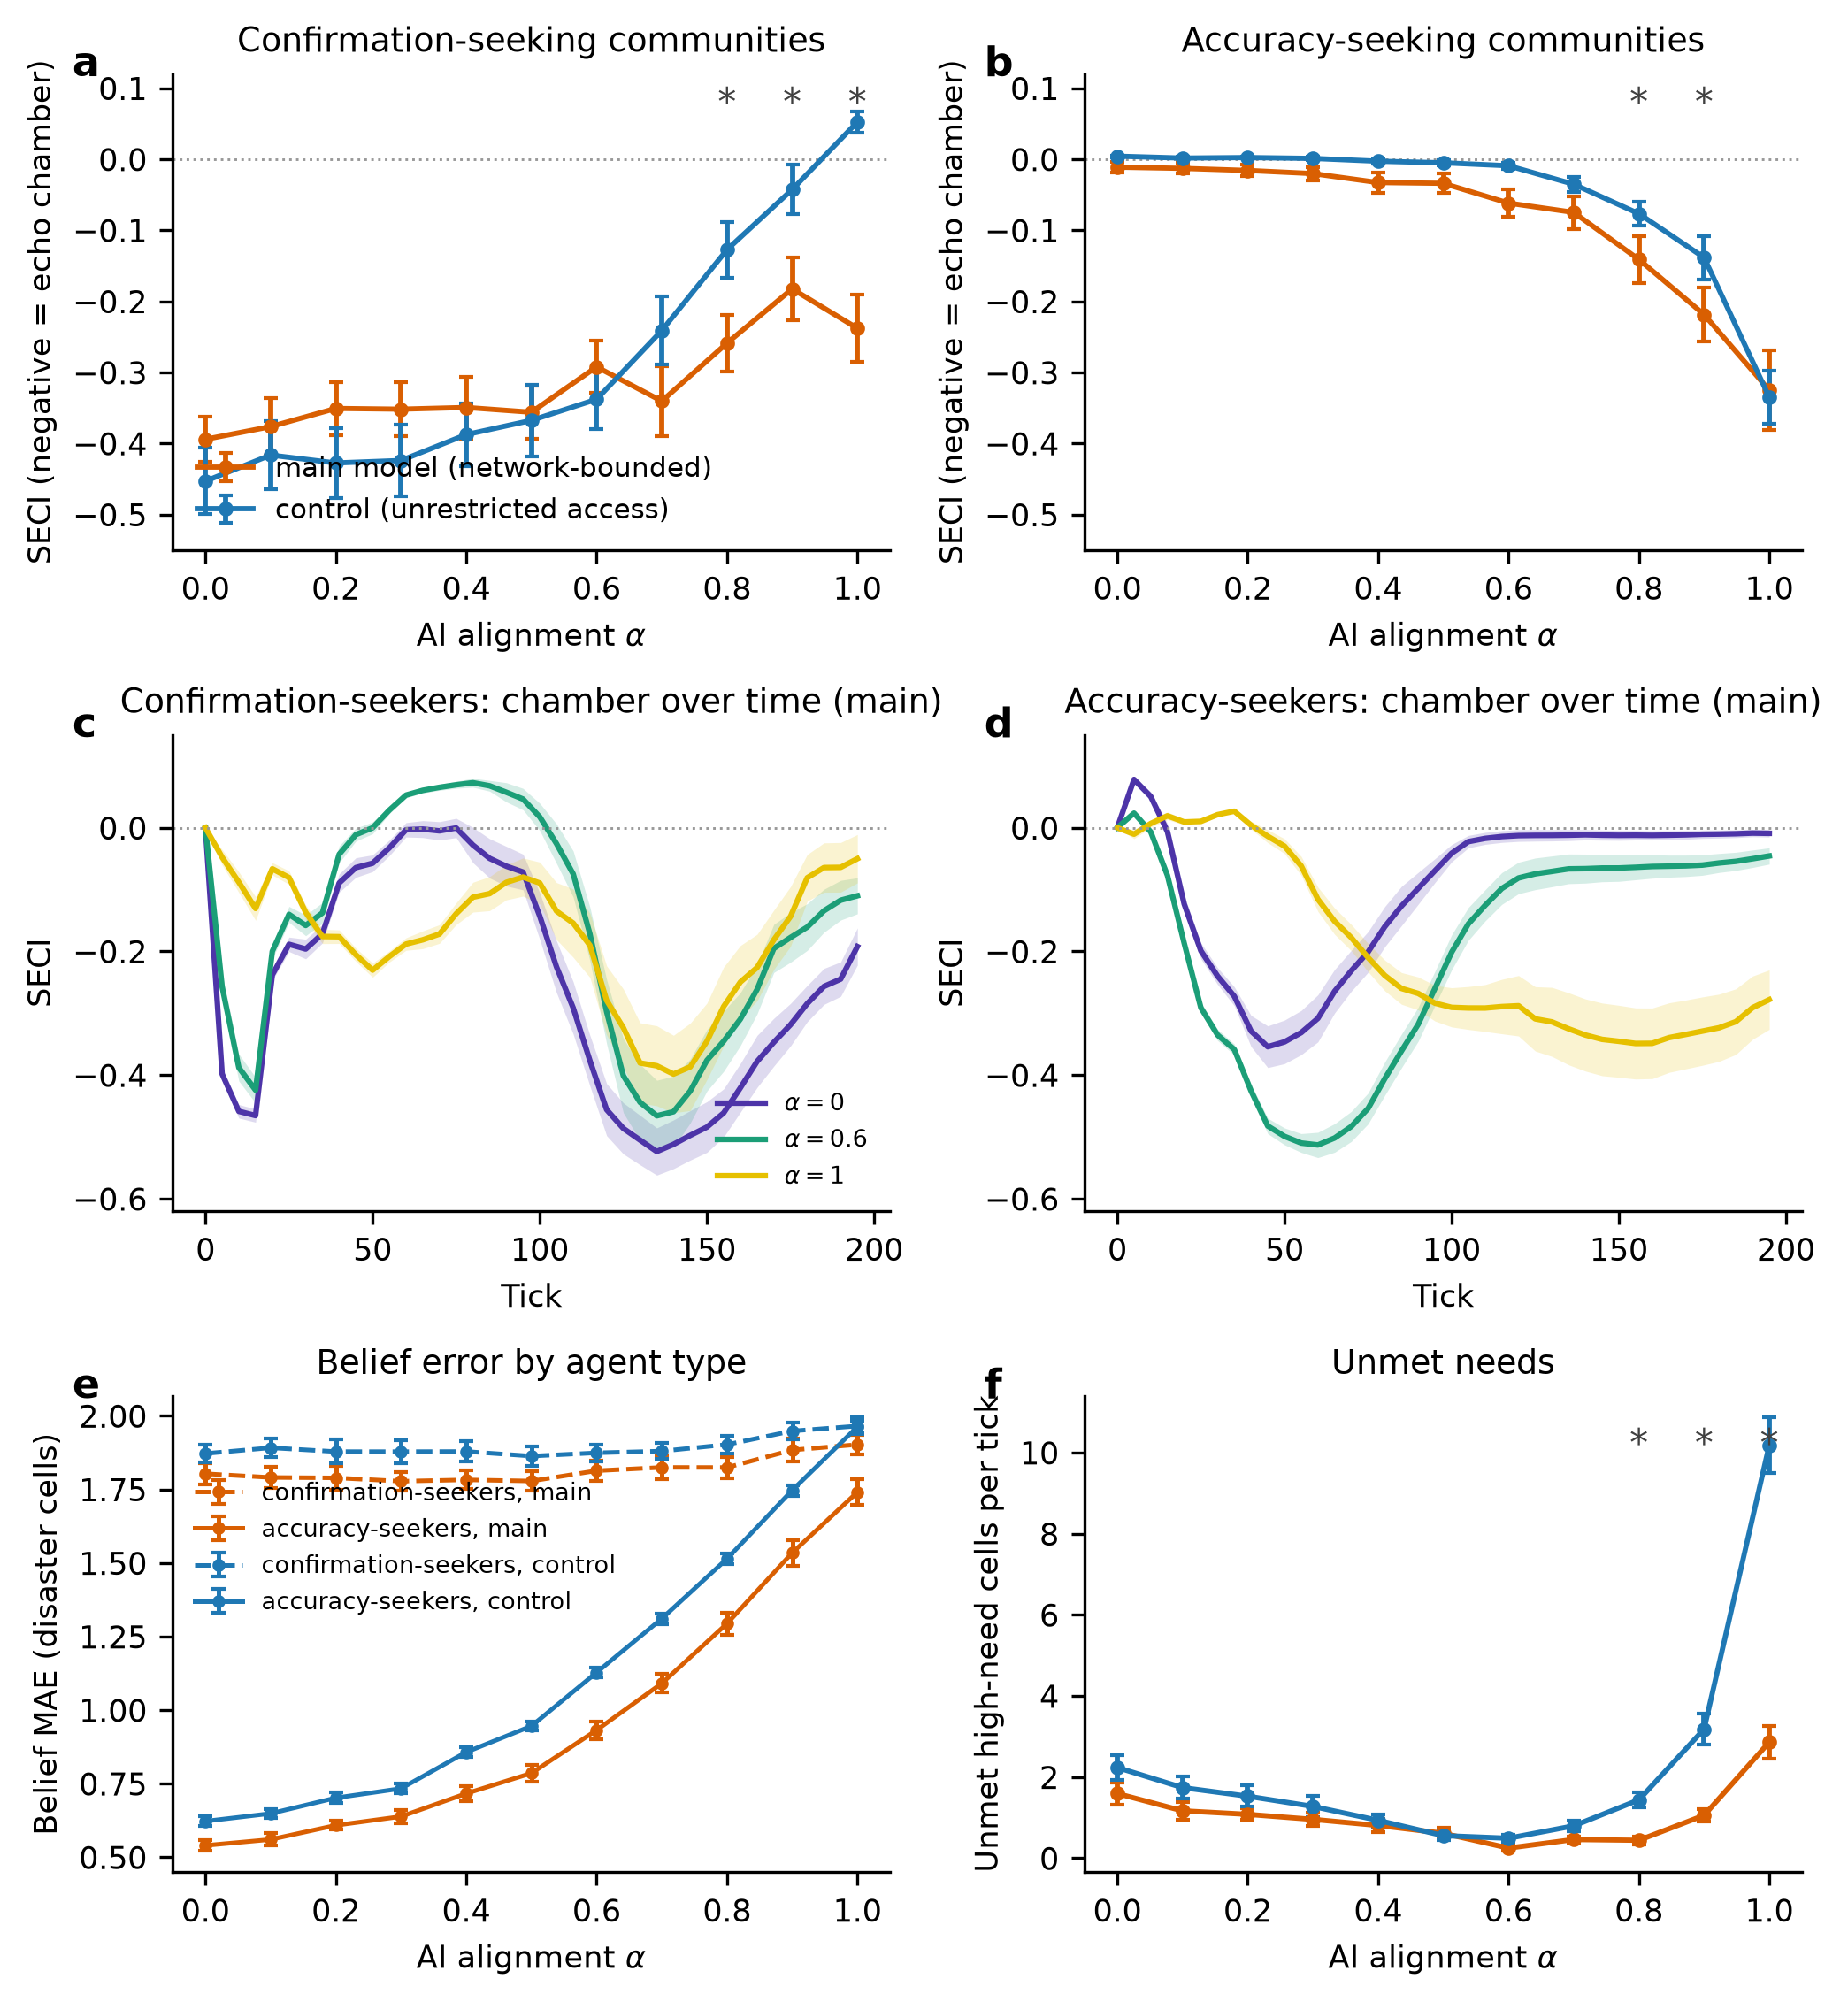
\includegraphics[width=\textwidth]{fig2_configuration.png}
\caption{Configuration comparison across the primary alignment sweep (steady-state means $\pm$ s.e.m., $N=20$ seed-paired replications; negative SECI = echo chamber). \textbf{a}, Social Echo Chamber Index of the confirmation-seeking (exploitative) communities: unrestricted access (blue) dissolves the chamber at high alignment while network-bounded access (orange) preserves it at every $\alpha$. \textbf{b}, The accuracy-seeking (exploratory) communities converge with alignment in both configurations. \textbf{c}, Belief error by agent type: the accuracy cost of alignment falls on the accuracy-seekers (solid), while the confirmation-seekers' error is flat at $\approx 1.8$ (dashed). \textbf{d}, Unmet high-need cells per tick: the operational optimum is interior in both configurations, and bounded access buffers the collapse at $\alpha=1$. Asterisks mark $\alpha$ levels at which the paired main$-$control contrast is significant after Holm correction ($N=50$ boundary replications for $\alpha \geq 0.8$; SI Appendix, Table~S1).}\label{fig:comparison}
\end{figure}

\subsection{Confirming AI harms accuracy-seekers by starvation, and the alignment optimum is interior}\label{sec:claim2}

The accuracy cost of alignment falls entirely on the accuracy-seekers (Fig.~\ref{fig:comparison}c). Their belief error grows from $0.54 \pm 0.02$ at $\alpha=0$ to $1.74 \pm 0.04$ at $\alpha=1$ under the main model (0.62 to 1.96 in the control), while the confirmation-seekers' error stays flat at $\approx 1.8$ at every alignment level: agents who accept only belief-consistent information are already impervious to reports, so a confirming AI cannot make them much worse. The dose--response is smooth at every step of the sweep---the delivered confirmation dose is linear in $\alpha$ by construction (manipulation check in Materials and Methods)---with no threshold at which harm switches on. The mechanism is starvation, not persuasion: a maximally confirming AI echoes the accuracy-seekers' mostly empty priors back at them, so they stop acquiring disaster knowledge, and their pool of informative beliefs collapses from 113 to 29 cells per agent (SI Appendix, Fig.~S2). Part of the deepening of their community chamber under alignment is therefore loss of belief diversity by emptying, not convergence on a shared false narrative. Over the run, alignment changes the chamber's lifecycle far more than its depth: the accuracy-seekers' communities enter a chamber in every replication at every alignment level, with peak depths in a narrow band ($-0.38$ to $-0.50$), but whether it dissolves again collapses with the dose---in 300-tick constant-policy runs, 17 of 20 replications dissolve their chamber under a truthful AI (median dissolution near tick 90) against 12 of 20 at $\alpha=0.8$ and 3 of 20 at $\alpha=1$ (SI Appendix, Fig.~S1 and Table~S11). The harm of alignment is not deeper echo chambers; it is chambers that no longer dissolve.

Because a truthful AI leaves the confirmation-seekers' social chamber standing (Fig.~\ref{fig:comparison}a) while a confirming AI starves the accuracy-seekers, the two failure modes penalize opposite ends of the alignment axis, and the total-bubble composite is minimized in the interior: $\alpha^{*} = 0.6$ for 7 of 12 composite definitions in the main model, with the remaining variants between 0.1 and 0.3 (Fig.~\ref{fig:goldilocks}a; sensitivity across all definitions in SI Appendix, Table~S2). The optimum is interior in the control as well (bubble composites at 0.8--0.9); an earlier corner solution at full confirmation was an artifact of a near-step delivered dose, as the single-mechanism rounding ablation attributes (SI Appendix, Table~S2). The operational optimum coincides: unmet high-need cells fall from 1.59 per tick at $\alpha=0$ to 0.25 at $\alpha=0.6$ before rising to 2.86 at $\alpha=1$ (Fig.~\ref{fig:comparison}d), with significant U-curvature on unmet needs, the population served-information index, and accuracy-seekers' precision (SI Appendix, Table~S6). The population layer tells the same story from the information side: the diversity of AI-served information is U-shaped in $\alpha$ in both configurations, shallowest near $\alpha=0.7$---society's served information environment is most diverse at intermediate alignment, exactly where operations perform best (SI Appendix, Fig.~S5).

\begin{figure}[t]
\centering
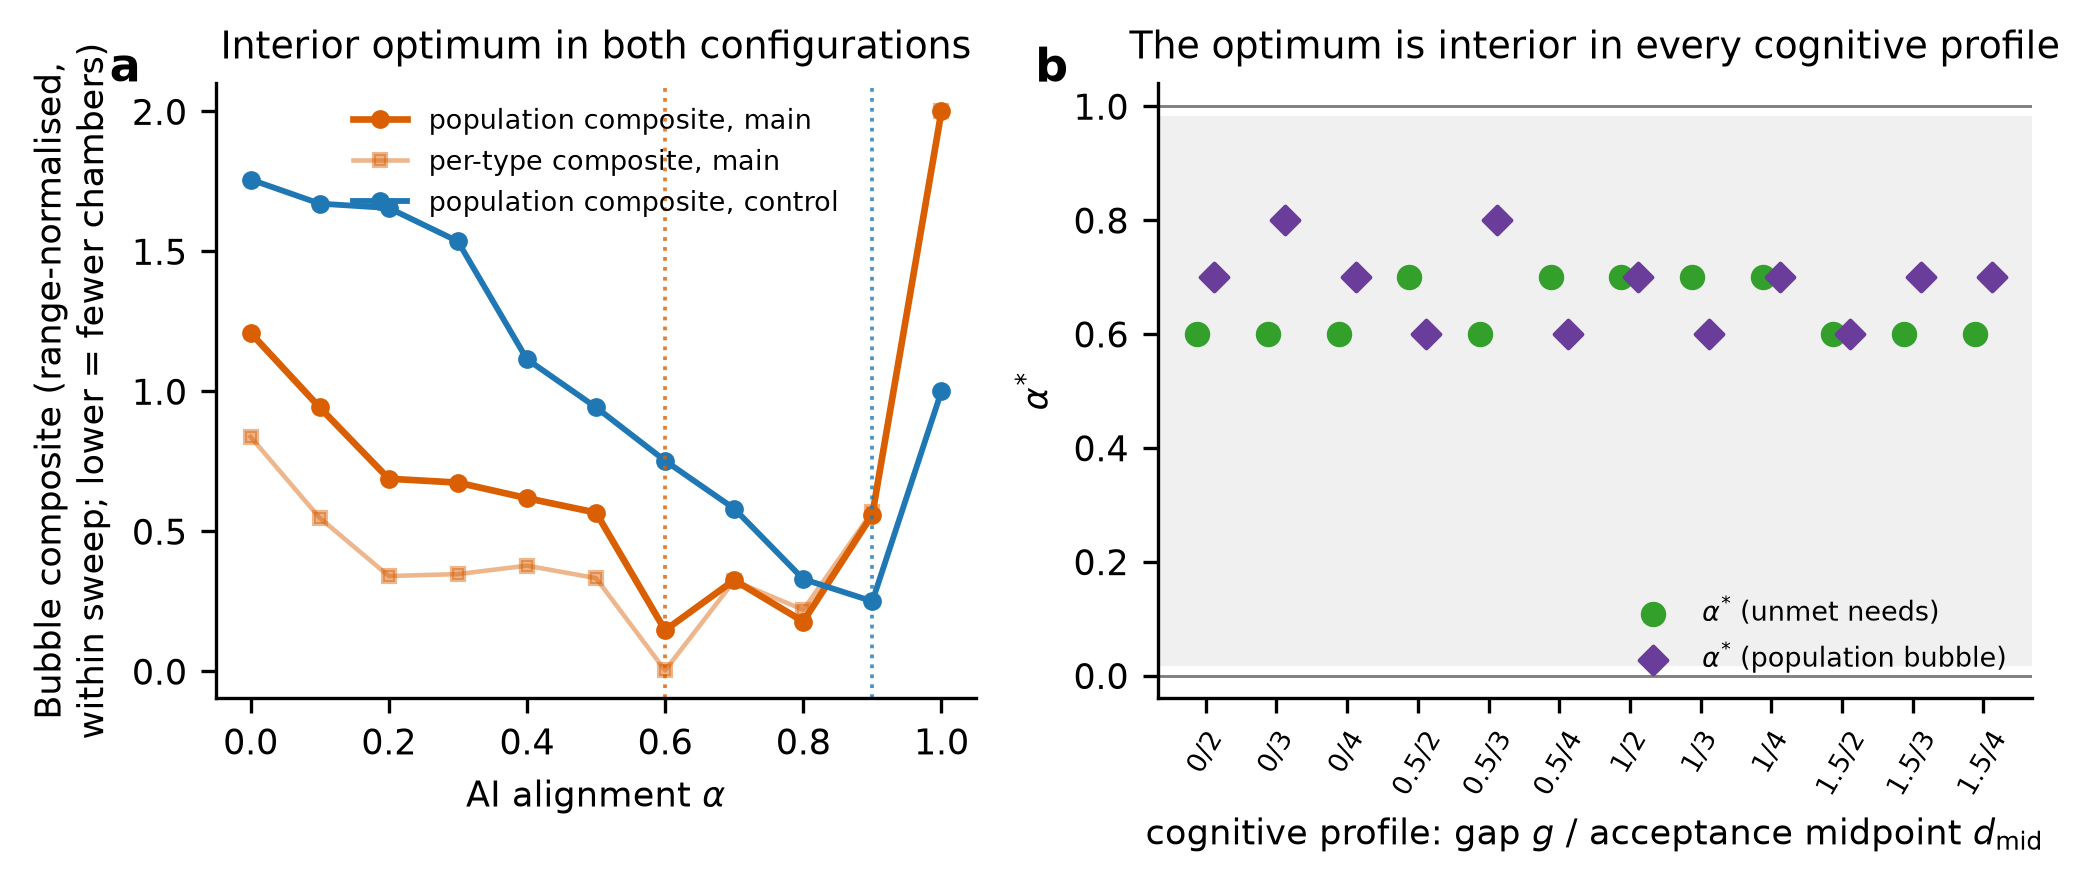
\includegraphics[width=\textwidth]{fig3_goldilocks.png}
\caption{The interior alignment optimum and its robustness. \textbf{a}, Bubble composite $|\mathrm{SECI}| + |\mathrm{AECI\mbox{-}IE}|$ (population level, range-normalized within each sweep; per-type variant overlaid) against $\alpha$: the optimum is interior in both configurations (dotted lines mark each configuration's $\alpha^{*}$; locations, not composite values, are compared across configurations). $\alpha^{*} = 0.6$ for 7 of 12 composite definitions in the main model (SI Appendix, Table~S2). \textbf{b}, The operational optimum ($\alpha^{*}$ of unmet needs, green) and the population bubble optimum (purple) across all twelve cognitive-profile cells of the gap sweep (cognitive gap $g \times$ acceptance midpoint $d_{\mathrm{mid}}$, $2{,}640$ runs): every cell places both optima strictly in the interior (0.6--0.8)---the interior optimum is a structural property of the information ecosystem, not a knife-edge of the assumed cognitive mix.}\label{fig:goldilocks}
\end{figure}

\subsection{The feedback loop captures confirmation-seekers, and making disconfirmation salient backfires into social retrenchment}\label{sec:claim3}

A confirming AI progressively captures the queries of precisely the agents it is tuned to satisfy. As $\alpha$ rises, the confirmation-seekers' AI share of queries climbs from 0.54 to 0.69 while their trust in the AI stays flat at $\approx 0.47$ (SI Appendix, Fig.~S3): the capture runs through the confirmation reward on accepted reports, not through growing confidence in the source. Capture also accelerates: sustained AI-majority reliance onsets at tick $59 \pm 2$ under a truthful AI but by tick $3 \pm 1$ from $\alpha=0.8$ upward, closing the loop before any verification signal can accumulate (SI Appendix, Table~S11). Accuracy-seekers are not captured---their AI share saturates near 0.60 from mid-alignment---but the heaviest AI users among them freeze: their belief-revision activity locks in (AECI-LockIn from $-0.01$ to $-0.13$; SI Appendix, Fig.~S2). Critically, accuracy-seekers never learn to distrust a confirming AI: their AI trust declines only from 0.88 to 0.84 across the entire sweep, because verification is dominated by the base rate of unaffected cells---in an instrumented probe, a fully confirming AI still passed verification on roughly 93\% of queried cells by echoing correct ``no impact'' priors (SI Appendix). This silent failure of verification-based correction is itself a finding, and it is robust: even when verification errors about disaster cells are weighted up to six times more heavily, trust only falls from 0.90 to 0.82 (SI Appendix, Table~S8).

A counterfactual that removes the base-rate dilution shows why the capture mechanism has no purely informational exit. With fully salience-weighted evaluation, the capture gradient disappears---the confirmation-seekers' AI share is flat at $\approx 0.5$ at every $\alpha$---but they do not become accurate; they retrench into their social network. At the truthful endpoint their community chamber \emph{deepens} (SECI $-0.52$ versus $-0.37$ without salience) and their relief precision falls (0.43 versus 0.57), with belief error unchanged (SI Appendix, Table~S8). Making disconfirmation salient ejects confirmation-seekers from the one truthful channel back into the social bubble: the demand for confirmation is conserved, and interventions that only penalize the AI channel relocate it.

A second counterfactual repairs the policy itself, switching a confirming AI to truthful at mid-run against constant-policy anchors on the same seeds. The social layer proves reversible: the accuracy-seekers' chamber dissolves in 18 of 19 replications in which it stood at the switch, and the confirmation-seekers' reliance falls back onto the truthful trajectory. The epistemic layer does not follow: 200 truthful ticks after the repair, the accuracy-seekers' belief pool remains depleted (102 versus 120 informative cells) and their belief error elevated (0.49 versus 0.41)---the starvation outlives the policy that caused it. The reverse switch is asymmetric: sycophancy imposed on an already-informed population neither starves it (pool 107 versus 30) nor re-forms the chamber. Alignment does its damage where beliefs are still forming---precisely the condition of disaster onset (SI Appendix, Fig.~S8 and Table~S11).

On the operational side, the same network boundedness that preserves the social chamber buffers the collapse of relief performance. At $\alpha=1$ the main model leaves 2.86 high-need cells unserved per tick against 10.18 in the control, and accuracy-seekers' targeting precision is 0.62 against 0.20 (paired $\Delta$unmet $-6.56$, Holm $p \approx 6\times10^{-17}$; SI Appendix, Table~S1); mobility and trusted local reports keep part of every agent's reward signal grounded in observation that no degree of AI confirmation can distort. Finally, the interior optimum that this feedback loop produces is not a knife-edge of the assumed population: across a $4 \times 3$ grid of cognitive profiles varying the gap between the two types and the population's acceptance midpoint, the operational and population-bubble optima are interior in every cell (0.6--0.8; Fig.~\ref{fig:goldilocks}b), and all headline mechanisms hold under perturbations of population size (100--500), network generator, AI supply (1--10), and verification throughput (SI Appendix, Fig.~S7).

\subsection{Harms concentrate on the spatial periphery}\label{sec:claim4}

The first three findings operate at the level of types and communities; the fourth traces how the harm is distributed within the population. The belief-error gap between agents based far from and near to the disaster widens with alignment, from $+0.12$ at $\alpha=0$ to $+0.33$ at $\alpha=1$ (Fig.~\ref{fig:periphery}a): agents remote from the events, who depend almost entirely on mediated reports, absorb most of the accuracy loss that confirmation produces. The behavioral consequence is withdrawal from the response: the far$-$near gap in contributed relief grows from $-1.8$ to $-6.6$ tokens with $\alpha$ (Fig.~\ref{fig:periphery}b)---the remote quartile does not merely become less accurate, it progressively stops sending assistance. Both gaps are absent at every $\alpha$ in the immobile control, where position carries no informational meaning: the structural null confirms that the gradient is produced by who can observe and verify, not by the AI policy itself. Network position offers no comparable protection---the belief-error differences between high- and low-betweenness agents remain small at every alignment level (SI Appendix, Table~S3). The harms of a confirming AI are spatially, not topologically, structured: they fall on those who cannot check reports against first-hand observation, regardless of how well connected they are---precisely the position of the remote coordination hubs that dominate data-driven crisis response \citep{comes2020coordination,coleman2024weaving}. The gaps also accumulate rather than equilibrate: at full alignment both are still widening when the run ends, so the reported steady-state gaps are conservative lower bounds on the harm a longer crisis would produce (SI Appendix, Fig.~S4).

\begin{figure}[t]
\centering
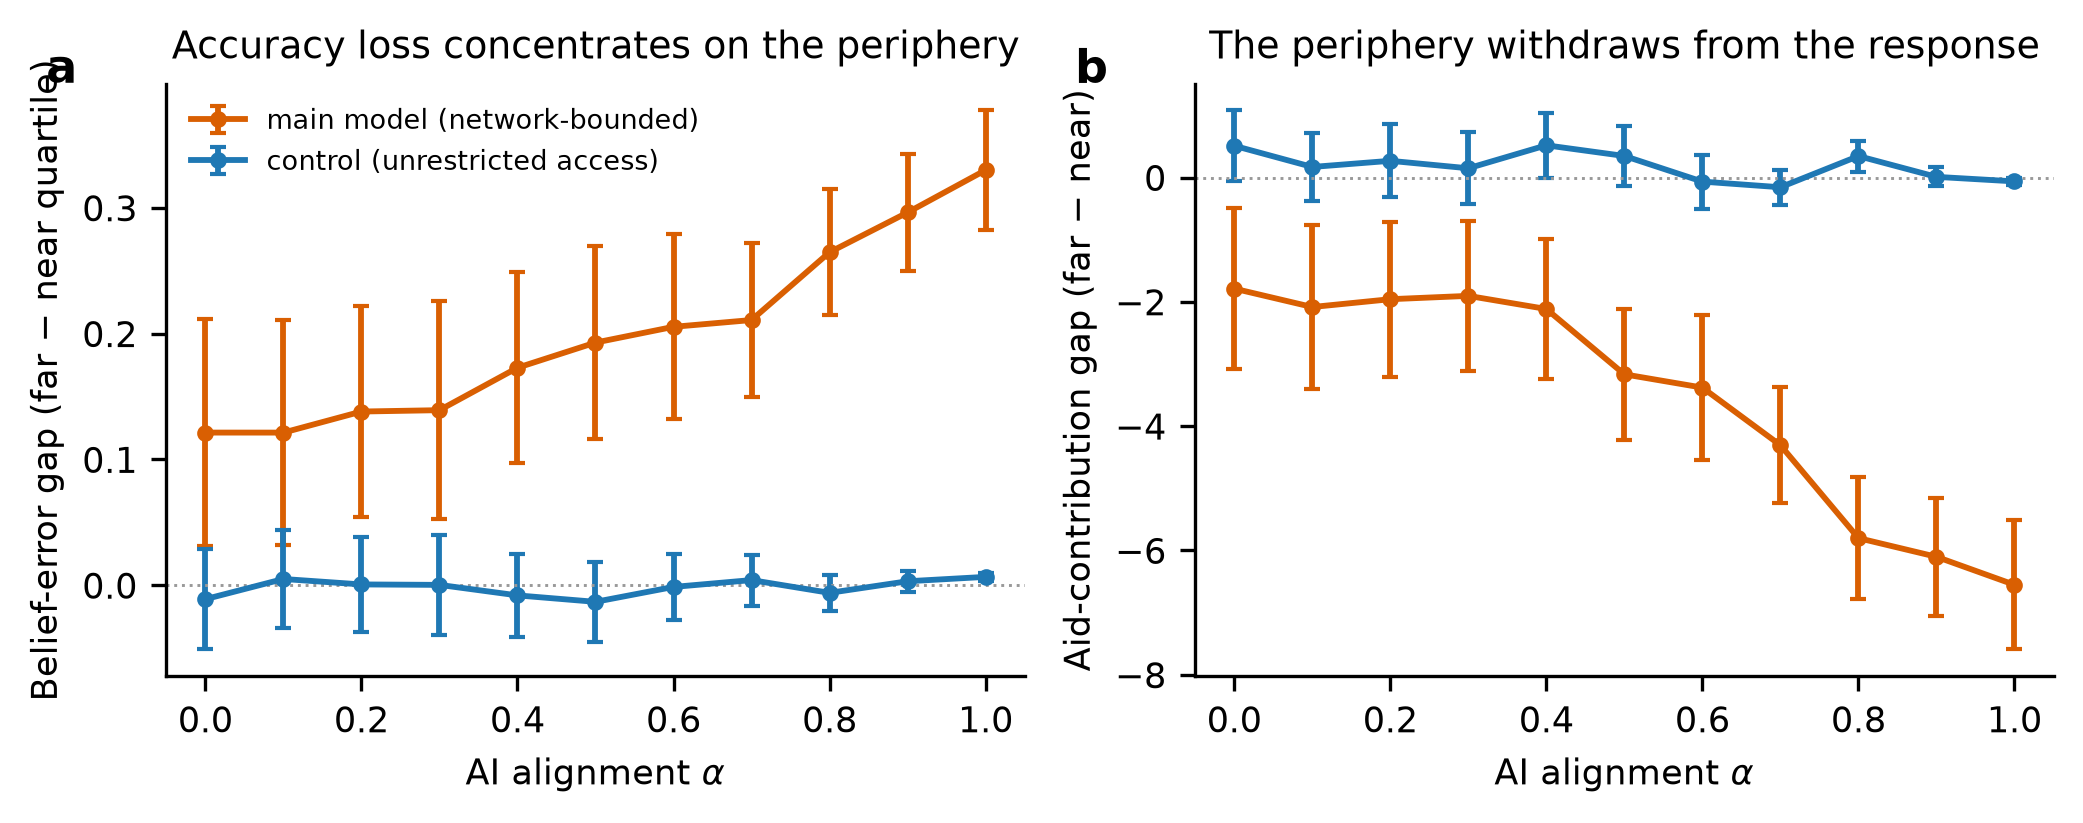
\includegraphics[width=\textwidth]{fig4_periphery.png}
\caption{Distribution of alignment harms across space (steady-state means $\pm$ s.e.m., $N=20$). \textbf{a}, Belief-error gap between the furthest and nearest quartile of agents by distance to the epicenter, against $\alpha$. \textbf{b}, Gap in contributed relief between the same quartiles. In the main model (orange) both gaps widen with alignment; in the immobile control (blue) both are indistinguishable from zero at every $\alpha$ (structural null). Network-centrality decompositions in SI Appendix, Table~S3.}\label{fig:periphery}
\end{figure}

\section{Discussion}\label{sec:discussion}

This paper asked whether an AI trained to please its users breaks echo chambers or reinforces them---and at what cost to the decisions that depend on the resulting beliefs. The answer replaces a single dose--response with a mechanism map. A sycophantic AI harms a networked population through two distinct, type-specific channels: it \emph{captures} confirmation-seekers, whose reliance rises with alignment while their trust never moves, and it \emph{starves} accuracy-seekers, whose supply of informative reports dries up until their beliefs freeze. Whether these individual-level mechanisms aggregate into community echo chambers is governed by a variable invisible at the dyadic level---the structure of who can query whom. The dyadic human--AI amplification documented experimentally \citep{glickman2024human} reproduces inside the model (SI Appendix, Fig.~S6), yet its population consequence is conditional: unrestricted access converts alignment harm into operational collapse without community chambers, while network-bounded access preserves the chambers and buffers operations. This parallels the classic result that network structure reverses the effect of social influence on crowd accuracy \citep{lorenz2011social,becker2017network}, and it implies that collective epistemic risk assessments of AI require network-level analysis: a model without structural constraints on access would have concluded that confirmation dissolves echo chambers.

The interior optimum ($\alpha^{*}=0.6$, robust across composite definitions, both configurations, and every cognitive profile tested) is a descriptive property of the trade-off between a truthful AI that goes unheeded by confirmation-seekers and a confirming AI that starves accuracy-seekers. It is not a design recommendation to build mildly sycophantic systems. The same adoption that intermediate alignment purchases through confirmation can be pursued through routes that do not distort content: communicating uncertainty, transparency about sources, and active support for verification \citep{glikson2020human,lee2004trust}. What the optimum's existence does establish is that the two endpoints most often argued for---maximal truthfulness as safety, maximal helpfulness as usability---are both dominated in operational terms, and that where a deployed system should sit depends on the social structure it enters, not only on the system.

The salience counterfactual sharpens the design lesson. The intuitive repair for capture---make disagreement between the AI and reality salient in evaluation---removes the capture gradient but produces social retrenchment: confirmation-seekers leave the truthful channel and deepen their community chamber, ending with worse targeting precision than under the unrepaired system. The demand for confirmation is a property of the users, not of the channel; interventions that only penalize one source relocate that demand to whichever source still supplies it. Effective intervention must therefore widen access to verifiable information---independent situation reports, deliberate exposure to first-hand observers---rather than merely punishing the confirming source. The same logic reframes monitoring: because operational degradation is gradual while community-level convergence deepens silently, dashboards that track individual accuracy and aggregate performance will miss the failure mode that matters; belief convergence within communities, reported per cognitive style, is the leading indicator. The reversal experiment adds a second monitoring lesson: after an intervention, recovery of the convergence index does not certify recovery of the knowledge base---the belief pool heals on a slower clock than the chamber, so a dashboard that declares victory when communities de-converge will do so while the population is still informationally starved. And because the damage is front-loaded into the belief-formation phase, the window for intervention is the onset of the crisis, not its aftermath.

A modeling commitment underpins the mechanism claims: the AI in this model is type-blind. It observes only the querier's revealed beliefs and applies one response rule to every caller; an ablation that redirects the confirmation target from the individual prior to the community consensus is behaviorally inert (SI Appendix, Table~S4). Every differential outcome---capture of one type, starvation of the other, the spatial gradient---therefore emerges from human acceptance windows, verification behavior, and reward learning interacting with network structure. This matters for external validity: the harms documented here require no user modeling, no personalization, and no intent on the AI side, only a policy that tilts toward agreement applied to a population that differs in how it seeks information.

Several limitations bound these conclusions. The alignment parameter is a reduced form for the drift produced by preference-based training \citep{sharma2023sycophancy}, not a model of any deployed system, and no quantitative claim---including the location of $\alpha^{*}$---transfers directly to real platforms. The hazard is stylized and the population small, though the findings are stable from 100 to 500 agents, under an alternative network generator, from monopoly to ten-provider AI supply, and across verification throughput (SI Appendix, Fig.~S7). Verification operates through an exogenous situation-report channel; endogenizing it is a natural extension, as are heterogeneous or adaptive AI policies, including policies tuned toward truthfulness for remote users, which the periphery finding motivates. Disasters were chosen as the extreme case; the ingredients---high stakes under time pressure, non-stationary ground truth, delayed and noisy verification, access bounded by ties and position---recur in public-health emergencies, financial contagion, and security operations, where the same mechanisms should operate more slowly and less visibly.

In sum: network-bounded information access is the structural precondition for AI-amplified community echo chambers; a confirming AI harms accuracy-seekers by starving them of information rather than persuading them, converting transient community chambers into ones that no longer dissolve and whose epistemic damage outlives the policy; the feedback loop of source selection captures confirmation-seekers, and suppressing that capture without widening verification backfires into social retrenchment; alignment harm is minimized at an interior level that is a property of the sociotechnical system; and the residual harm concentrates silently on those remote from the events. Trustworthy AI in urgent, high-stakes settings is a property of the system formed by the AI policy, the social network, and the distribution of verification opportunities---and it must be designed and monitored as such.

\section{Materials and Methods}\label{sec:methods}

\textbf{Model overview.} We develop an agent-based model of disaster response in which 100 human agents form beliefs about local disaster severity on a $30 \times 30$ grid, seek information from social contacts or from five AI agents, and dispatch relief accordingly. Each cell carries a severity level 0--5, initialized as a Gaussian decay from a random epicenter and perturbed by stochastic shocks (probability 0.10, magnitude $\pm 2$), producing a non-stationary ground truth that forces ongoing information seeking. Agents belong to one of two cognitive types in equal shares \citep{march1991exploration}: \emph{exploitative} agents are confirmation-seeking, with a narrow acceptance window ($D = 2.0$) and steep acceptance sensitivity ($\delta = 3.5$); \emph{exploratory} agents are accuracy-seeking ($D = 4.0$, $\delta = 1.2$). A report at distance $d$ from the current belief is accepted with probability $D_{\mathrm{eff}}^{\delta} / (d^{\delta} + D_{\mathrm{eff}}^{\delta})$, where trust widens $D_{\mathrm{eff}}$ for friends; accepted reports update beliefs by precision-weighted Bayesian revision, generalizing bounded-confidence models \citep{deffuant2000mixing,hegselmann2002opinion}. Agents select among querying a friend, querying the AI, or acting, via $\epsilon$-greedy Q-learning; relief outcomes return as delayed rewards (15--25 ticks). Report evaluations differ by type: exploitative agents score sources for \emph{confirmation} against their trusted network's consensus belief when defined, their own prior otherwise; exploratory agents score sources for \emph{accuracy} against external verification, which arrives through an exogenous situation-report channel with delay and noise. Because most queried cells are truly unaffected, per-cell verification is base-rate dominated; a salience weight $s \in [0,1]$ (default 0; counterfactual $s=1$) interpolates toward severity-weighted evaluation of both channels.

\textbf{AI alignment.} A queried AI responds with $r = (1-\alpha)\,t + \alpha\,b$, where $t$ is the cell's severity as available to the AI (15\% of the grid sensed per tick, with $\alpha$-independent noise and $\alpha$-independent extrapolation for unsensed cells) and $b$ is the \emph{querier's own current belief}, for both agent types. The delivered report is discretized by stochastic rounding, making the delivered confirmation dose linear in $\alpha$ in expectation (manipulation check: measured effective $\alpha$ is linear in nominal $\alpha$); a deterministic-rounding ablation shows that the near-step dose of naive rounding, not any behavioral mechanism, produced earlier corner solutions (SI Appendix, Table~S2). The AI is non-adaptive and type-blind, so all learning dynamics are attributable to the human agents. $\alpha$ is a reduced-form representation of the outcome of preference-based training \citep{christiano2017deep,ouyang2022training,sharma2023sycophancy}, not of the training process.

\textbf{Configurations.} The \emph{main model} enables three structural mechanisms: agents move following the returner--explorer dichotomy of human mobility, communities are spatially embedded and connected by sparse weak-tie bridges \citep{granovetter1973strength}, and human queries are network-gated (trust-weighted over friends, with probability 0.1 of two-hop reach). The \emph{control} disables all three: immobile agents, disconnected communities detached from space, and global query access. All other mechanisms and parameters are identical (SI Appendix, Table~S7).

\textbf{Metrics.} SECI compares the belief variance within each social community (beliefs at severity $\geq 1$, the informative L1+ pool) to global belief variance, with asymmetric normalization to $[-1, 1]$; negative values mark an echo chamber; community values are averaged within type, and a population-level variant pools all communities. AECI-IE applies the identical variance-ratio construction to the report levels a community receives from the AI channel during the metrics window, against the diversity of that channel's global served pool (a channel-baseline construction; the human-channel counterpart SECI-IE serves as a consistency check, and retired variants are reported in SI Appendix, Table~S2). AECI-LockIn measures the freezing of belief revision among AI-heavy agents; the L1+ pool size measures belief starvation. Accuracy and operations are measured by MAE over disaster cells, unmet needs (high-need cells receiving no relief per tick), and targeting precision. Composites for locating $\alpha^{*}$ range-normalize $|$SECI$|$ and $|$AECI-IE$|$ within a sweep; $\alpha^{*}$ is reported with its sensitivity across all 12 composite definitions.

\textbf{Design and statistics.} The primary experiment is a full factorial of 11 $\alpha$ levels $\times$ 2 configurations $\times$ 20 seed-paired replications of 200 ticks (steady state: last 75 ticks). Configuration effects are estimated as paired per-seed deltas with Holm-corrected confidence intervals, extended to $N=50$ replications at the boundary levels $\alpha \in \{0.8, 0.9, 1.0\}$; dose--response curvature is estimated by mixed-effects regression of z-scored outcomes on $\alpha$, $\alpha^2$, configuration, and interactions with seed as grouping factor (SI Appendix, Tables~S1 and~S6). Supporting experiments: a $4 \times 3 \times 11$ cognitive-profile sweep ($2{,}640$ runs), single-mechanism ablations, a salience counterfactual, a robustness envelope over population size, network generator, AI supply, and verification probability, and a dyadic docking experiment reproducing the human--AI amplification of \citet{glickman2024human} (SI Appendix). Dynamics are quantified by per-replication lifecycle statistics---chamber formation and dissolution ticks (with hysteresis thresholds; dissolution right-censored at the horizon), persistence, and capture onset---and by an alignment-reversal experiment that switches $\alpha$ mid-run against constant-$\alpha$ anchors on the same seeds (SI Appendix). The model is implemented in Python (Mesa, NetworkX); all runs are seeded and reproducible, and figures are regenerated from archived outputs without re-simulation.

\backmatter

\bmhead{Supplementary information}
The SI Appendix contains the full ODD-style model specification, metric formalism, calibration table, supplementary figures S1--S8, and tables S1--S11, including the paired-contrast tables, the $\alpha^{*}$ sensitivity and ablation-attribution table, the regression table, the salience-counterfactual cells, the lifecycle and alignment-reversal statistics, and the transparency chain across model revisions.

\bmhead{Acknowledgements}
%% To be completed.

\section*{Declarations}

\bmhead{Funding} No funding sources provided support for this project.
\bmhead{Conflict of interest} The author declares no competing interests.
\bmhead{Data availability} All simulation outputs underlying the figures and tables are archived with the code repository (\texttt{results-mechfix/} and companion directories); a Zenodo DOI covering code and all results directories will be minted at submission.
\bmhead{Code availability} The full model, parameter files, and post-processing scripts are available at \url{https://github.com/tinacomes/DisasterAI}.

%% All cited keys resolve from References.bib. One placeholder remains
%% flagged inside References.bib: steinbrink2024transparency (unused here).
\bibliography{References}

\end{document}
